\documentclass[12pt, a4paper]{report}
\usepackage[utf8]{inputenc}
\usepackage{afterpage}
\usepackage{listings}
\usepackage{graphicx}
\graphicspath{ {imagenes/} }
\begin{document}
\begin{LARGE}
\begin{center}

Instituto Politécnico Nacional

\bigskip
\bigskip

Escuela Superior de Cómputo

\bigskip
\bigskip

Gonzalez Mora Javier

\bigskip
\bigskip

Sistemas operativos

\bigskip
\bigskip

2CM7


\end{center}
\end{LARGE}

\newpage

\begin{center}

Indice

\end{center}

\bigskip
\bigskip

\begin{flushleft}
Explicacion teorica .............................................................3

\bigskip

Programas utilizados...........................................................4

\bigskip

Desarrollo de la practica......................................................5

\bigskip

Errores y soluciones.............................................................9

\bigskip

\end{flushleft}

\bigskip
\bigskip

\bigskip

\newpage




\begin{center}

Practica 2

\end{center}

\begin{flushleft}


Escribir una cadena ya sea por interrupciones en la BIOS o directamente en la memoria de video.


\bigskip

En el primer caso una interrupcion del BIOS es un mecanismo que tienen las computadoras que detiene el ciclo de fetch para atender un evento solicitado y no solicitado.


\bigskip
Se usan para:
\begin{flushleft}
\begin{itemize}
\item Seguridad
\item Operaciones de entrada/salida
\item Proveer funciones del BIOS y del S.O.
\end{itemize}
\end{flushleft}

\bigskip

En el segundo caso se hace uso directo de la memoria de video, que es mediante la direccion B8000 por la cual se puede acceder y poder escribir el mensaje deseado.

\bigskip
\bigskip

\end{flushleft}




\newpage

\begin{center}
Programas utilizados y como fueron utilizados
\end{center}

\bigskip
\bigskip

\begin{flushleft}
\begin{itemize}
\item NASM: Se uso para poder compilar el codigo escrito a lenguaje maquina.
\item QEMU: Se uso para poder virtualizar la imagen ISO previamente creada.
\item genisoimage: Se uso para poder generar la imagen ISO, la cual fue creada con el codigo en NASM.
\end{itemize}
\end{flushleft}

\newpage

\begin{center}
Desarrollo de la practica
\end{center}

\bigskip
\bigskip



\begin{center}
Se hizo uso NASM para compilar el codigo del archivo bootloaderesc.asm que posteriormente se generaria un archivo bootloaderesc.bin. Lo que hace el bootloader es escribir mediante la interrupcion 10H una cadena con un mensaje, despues se rellena de ceros hasta una longitud de 512 bytes, despues se coloca el MAGICK NUMBER en la posición 521 y 522.

\bigskip
\bigskip

\begin{flushleft}
Codigo del bootloader que escribe en pantalla por medio de interrupcion:

\bigskip
\bigskip

\lstinputlisting{../../src/bootloaderesc.asm}
\end{flushleft}

\bigskip
\bigskip

\end{center}
\begin{center}

\bigskip
\bigskip

\newpage

Instruccion para compilar y generar el archivo.bin: nasm src/bootloaderesc.asm -f bin -o  bin/bootloaderesc.bin

\bigskip
\end{center}
\begin{center}
Se crea un disco con el cargador:

Se crea un floppy disk:

Instrucciones: 
\bigskip

dd if=/dev/zero of=imagenes/bootloaderesc.flp bs=1024 count=1440

\bigskip

dd if=bin/bootloaderesc.bin of=imagenes/bootloaderesc.flp seek=0 count=1 conv=notrunc

\bigskip

Se corre el bootloader

\bigskip

Instrucciones:

\bigskip

qemu-system-i386 -fda imagenes/bootloaderesc.flp

\bigskip

Pantalla de resultados haciendo uso de interrupciones:

\bigskip

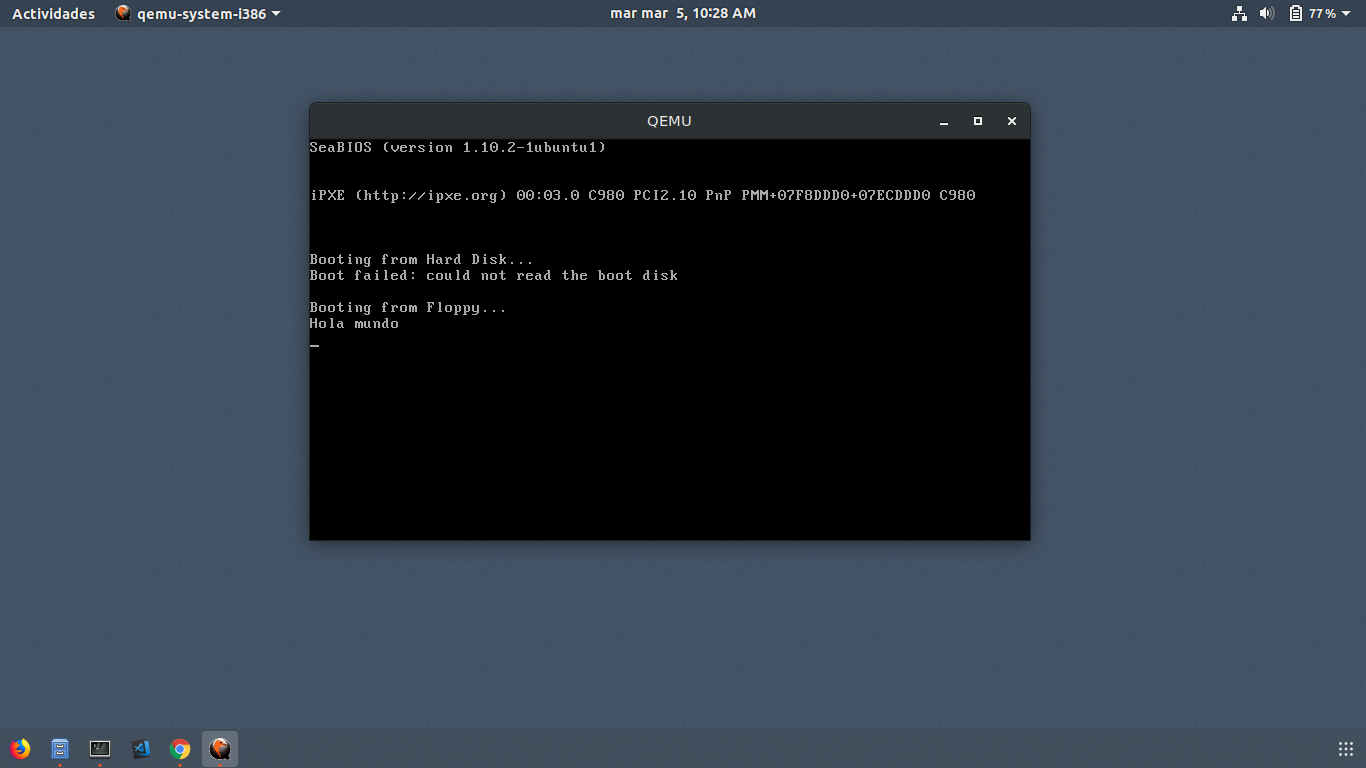
\includegraphics[scale=.3]{int1.png}

\bigskip

\end{center}

\newpage

\begin{center}
Se hizo uso NASM para compilar el codigo del archivo bootloaderlet.asm que posteriormente se generaria un archivo bootloaderlet.bin. Lo que hace el bootloader es escribir directamente en memoria de video haciendo uso de registros de proposito general caracter por caracter, despues se rellena de ceros hasta una longitud de 512 bytes, despues se coloca el MAGICK NUMBER en la posición 521 y 522.

\bigskip
\bigskip

\begin{flushleft}
Codigo del bootloader que escribe directamente en la memoria de video:

\bigskip
\bigskip

\lstinputlisting{../../src/bootloaderlet.asm}
\end{flushleft}


Instruccion para compilar y generar el archivo.bin: nasm src/bootloaderlet.asm -f bin -o  bin/bootloaderlet.bin

\bigskip
\end{center}
\begin{center}
Se crea un disco con el cargador:

Se crea un floppy disk:

Instrucciones: 
\bigskip

dd if=/dev/zero of=imagenes/bootloaderlet.flp bs=1024 count=1440

\bigskip

dd if=bin/bootloaderlet.bin of=imagenes/bootloaderlet.flp seek=0 count=1 conv=notrunc

\bigskip

Se corre el bootloader

\bigskip

Instrucciones:

\bigskip

qemu-system-i386 -fda imagenes/bootloaderlet.flp

\bigskip

Pantalla de resultados haciendo uso de la memoria de video:

\bigskip

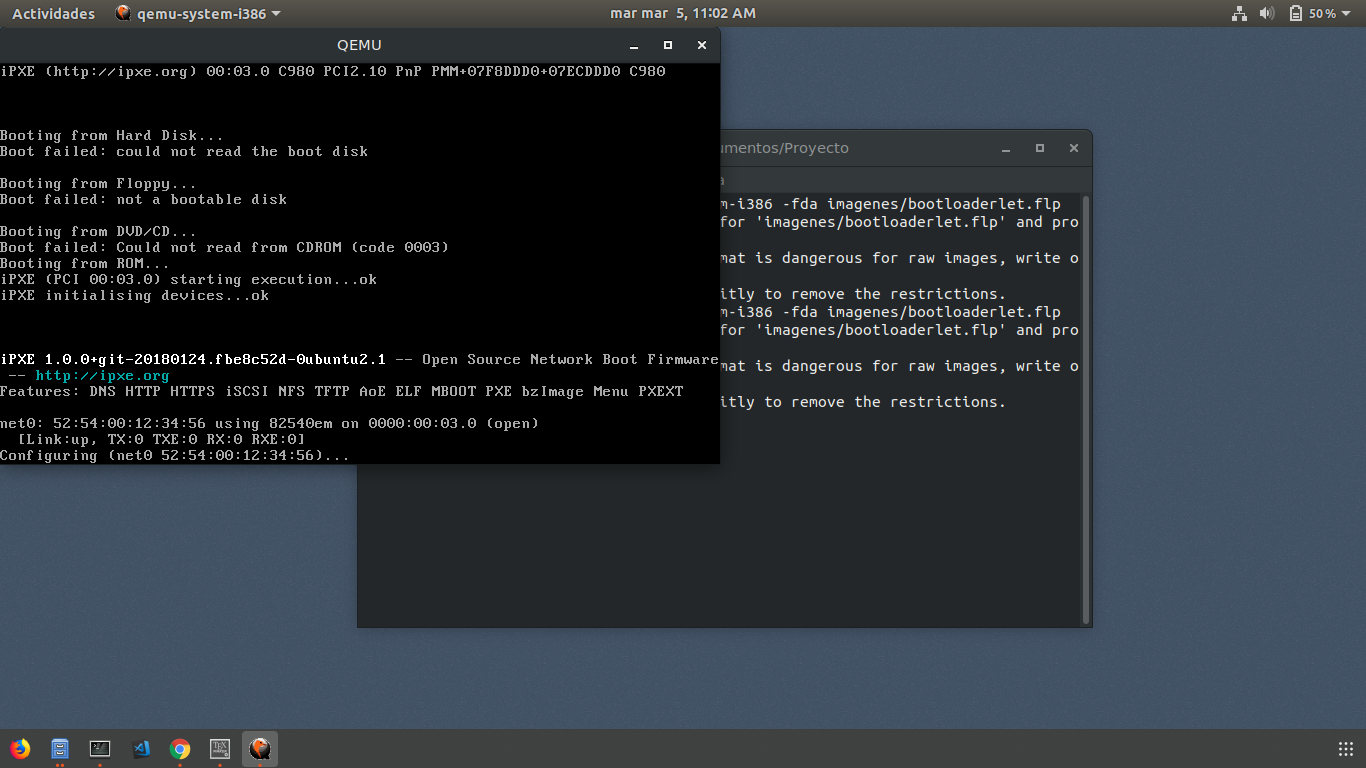
\includegraphics[scale=.3]{memoria.png}

\bigskip




\end{center}
\newpage



\begin{center}
Problemas que se presentaron: 

Ninguno


\bigskip

\end{center}

\end{document}